%%%%%%%%%%%%%%%%%%%%%%%%%%%%%%%%%%%%%%%%%%%%%%%%%%%%%%%%%%%%%%%%%%%%%%%
% Based on IEEE the conference template available                     %
% at https://www.ieee.org/conferences/publishing/templates.html       %
% Adapted for the Data Science Lab course at Politecnico di Torino    %
% by Giuseppe Attanasio, Flavio Giobergia                             %
% 2020, DataBase and Data Mining Group                                %
%%%%%%%%%%%%%%%%%%%%%%%%%%%%%%%%%%%%%%%%%%%%%%%%%%%%%%%%%%%%%%%%%%%%%%%

\documentclass[conference]{IEEEtran}
\usepackage{cite}
\usepackage{amsmath,amssymb,amsfonts}
\usepackage{algorithm}
\usepackage{algorithmic}
\usepackage{graphicx}
\usepackage{textcomp}
\usepackage{xcolor}
\usepackage{subfigure}

\begin{document}

\title{
Lab L6: Dynamic processes on graphs
}

\author{
    \IEEEauthorblockN{Emanuele Pietropaolo}
    \IEEEauthorblockA{
        \textit{Politecnico di Torino} \\
        Student id: s319501 \\
        emanuele.pietropaolo@studenti.polito.it
        }
}

\maketitle
\begin{abstract}
    A dynamical process is a mathematical model that describes the evolution of a system.
    %
    When run on a graph, it can model complex real-world scenarios such as pandemics or voter preferences.
    %
    In this context, the nodes represent the state of the system and the edges represent the possible transitions that the system can make. 
    %
    Simulating how such a system evolves over time can provide useful insights into how the modelled system behaves, more than analytical analyses can. 

    This paper presents different simulations of the \textit{Voter Model} on random graphs (\textit{Erdős-Rényi model}) and on $Z^2$ and $Z^3$ graphs to see how these types of graphs behave in different conditions, how the initial state and the size influence the time to reach consensus and the +1 consensus probability.

\end{abstract}

\section{Problem overview}

    The Voter Model is a mathematical model that describes a dynamic process.
    %
    It models the evolution of opinions in a group of people.  
    %
    As we simulate the Voter Model on to a graph, each node of the graph represents an individual and the edges between nodes represent the connection that each person has with the others.

    This report analyses some key questions about the dynamic of the process.
    %
    It analyses whether the dynamics converge to a final state, often referred to as consensus, and what are its characteristics.
    %
    It also analyses the influence of the initial conditions and the underlying graph structure on the dynamics of the system.

    % In this study, we aim to address several key questions related to the dynamics of our system. First and foremost, we seek to understand whether the dynamics of the system converge to a particular state or configuration. If convergence is observed, we are interested in characterizing the properties of the equilibrium point, often referred to as the consensus state. Furthermore, we aim to investigate the influence of the initial conditions on the system’s dynamics. Do different initial states lead to different trajectories or final states? Lastly, we consider the role of the underlying graph structure in shaping the system’s dynamics. How does the topology of the graph, including its connectivity and clustering, impact the evolution of the system? These questions form the basis of our investigation and guide our analysis of the system’s behavior.

\section{Proposed approach}

    The Voter Model suits the situation where there are two different opinions and individuals can be influenced by what their connections think about them. 
    %
    The opinion that a person has is represented by a state variable that can take two values: $ x_v(t) \in \{-1,1\}$.
    %
    The change in opinion is modelled as an event where a node wakes up and changes its state variable by copying the state variable of one of its neighbours, following the formula:

    \begin{center}
        \begin{math}
            x_v(t_v^+) = x_w(t_v^-)
        \end{math}
    \end{center}

    Simulating the voter model over a graph involves several steps. 
    %
    First, you need to generate the graph you want to use, and then you start modelling the events that cause the system to evolve.

    \subsection{Data structure for the graph}

        A \textbf{dictionary} was used to implement the graph. 
        %
        Each node is accessible by an index and contains a nested disctionary where the state variable and the list of neighbours are stored. 

        Each state variable is initialised according to the probability of being in the $+1$ state, this probability was called the \textit{bias probability}. 

    \subsection{Algorithm to generate samples of $G(n,p)$ graphs}
    
        One of the most common types of graph is the random graph. 
        %
        It is described by a probability distribution or random process that generates it. 
        %
        In fact, its number of edges depends on a stochastic process that connects the nodes based on a probability, the \textit{edge probability}. 
        %
        The model that almost exclusively describes a random graph is the Erdős Rényi (ER) model. 

        When the ER graph is generated, the dictionary is initialised with the desired number of nodes, without first connecting them. 
        %
        Then, to create the connection according to the edge probability, one of two methods are used based on the difference (in terms of factor of 10) between the number of nodes and the edge probability:
        \begin{itemize}
            \item \textbf{Bernoulli experiment for each pair of nodes}: this method involves iterating over all the nodes, and for each one iterates over all the nodes not yet seen. 
            %
            This method then creates an edge between a pair of vertices based on the \textit{bias probability}.
            %
            This algorithm has a complexity of $O(n^2)$, but tends to be $O(nlog(n))$ because the second for loop is decreasing in time.

            \item \textbf{Take advantage of low edge probability}: if p can be considered small before the number of nodes, the number of expected edges ($m$) that the graph will have can be calculated by the formula:
            \begin{center}
                \begin{math}
                    (n \cdot (n-1)\cdot p)/2 
                \end{math}            
            \end{center}        
            where $p$ is the \textit{edge probability}. 
            %
            Then, for each edge, two random nodes that are not already connected are selected and connected.
            %
            This algorithm has complexity $O(m)$, which tends to $O(n)$ for small values of $p$.
        \end{itemize}

    \subsection{Algorithm to generate samples of $Z^k$ graphs}

        A graph can also be a \textit{k-dimensional lattice}, where each node has an edge with all the nearest nodes in space. 
        %
        In this paper are explored the $Z^2$ and $Z^3$ grids. 
        %
        The nodes of these graphs are arranged in such a way so that they form a 2D or 3D grid respectively, and where a node has all edges perpendicular and parallel to the others.

        To generate a finite $Z^k$ graph, is first calculated the dimension of the grid to obtain a lattice with at least the desired number of nodes.
        %
        Then the dictionary is instantiated with this dimension and each node index is a tuple representing the coordinates (a pair or a triple respectively).
        %
        Finally, the edges are created to connect each node to its nearest neighbour. 

    \subsection{The unfolding of events}

        As mentioned above, the dynamic evolves through wake-up events.
        %
        Each event is associated with a particular node, which picks a random neighbour and copies its state variable. 
        %
        Since each wake-up event is independent and occurs with a known frequency, it is assumed that the wake-up process for each node follows a Poisson distribution with $\lambda = 1$. 
        %
        This implies that the wake-up process for the whole graph can be modelled as a process following a Poisson distribution with $\lambda =$ number of nodes in the graph.
        %
        The time between events is generated from an exponential distribution and each time a random node is chosen to wake up.

        Knowing that on finite graph the simulation always reach consensus, we can stop the simulation when it's reached. 

    \subsection{Simulation parameters}
        
    Several types of simulations are performed.
    
    \textbf{ER graphs} are simulated on a different range of nodes between $1000$ and $10000$ nodes. More precisely with $1000$, $4000$ and $6000$ nodes.
    %
    The edge probability is always set to be $p_e = n/10$.
    %
    Each range of graph is simulated with different \textit{bias probability} $(p_1)$, where $p_1$ can take values $\{0.51, 0.55, 0.6, 0.7\}$.

    \textbf{$Z^k$ graphs} are simulated on a different range of nodes between $100$ and $1000$ nodes, each time with \textit{bias probability} $p_1 = 0.51$.

    For each type of simulation, the confidence level is calculated in order to obtain a more reliable result, and it is accepted when it reaches a certain accuracy.
    %
    For computational reasons, both have been set at 80\%.

\section{Results}

    Tab. \ref{tab:all_graphs} shows the average time to reach consensus for every discussed type of graph when $n = 1000$ and $p_1 = 0.51$.
    %
    It can be seen that the $Z^2$ graph has a significantly higher average time to reach consensus. This can be explained by the low average degree of this graph type. 

    \begin{table}[!ht]
        \centering
        \caption{Average time to reach consensus with $n = 1000$ and $p_1=0.51$}
        \label{tab:all_graphs}
        \begin{tabular}{|c|c|c|c|}
        \hline
                & ER       & Z2        & Z3       \\ \hline
        Time & 589,1798 & 2054,6865 & 856,7241 \\ \hline
        \end{tabular}
    \end{table}
    

    \subsection{Erdős Rényi graphs} 

        \begin{figure}[!ht]
            \centering
            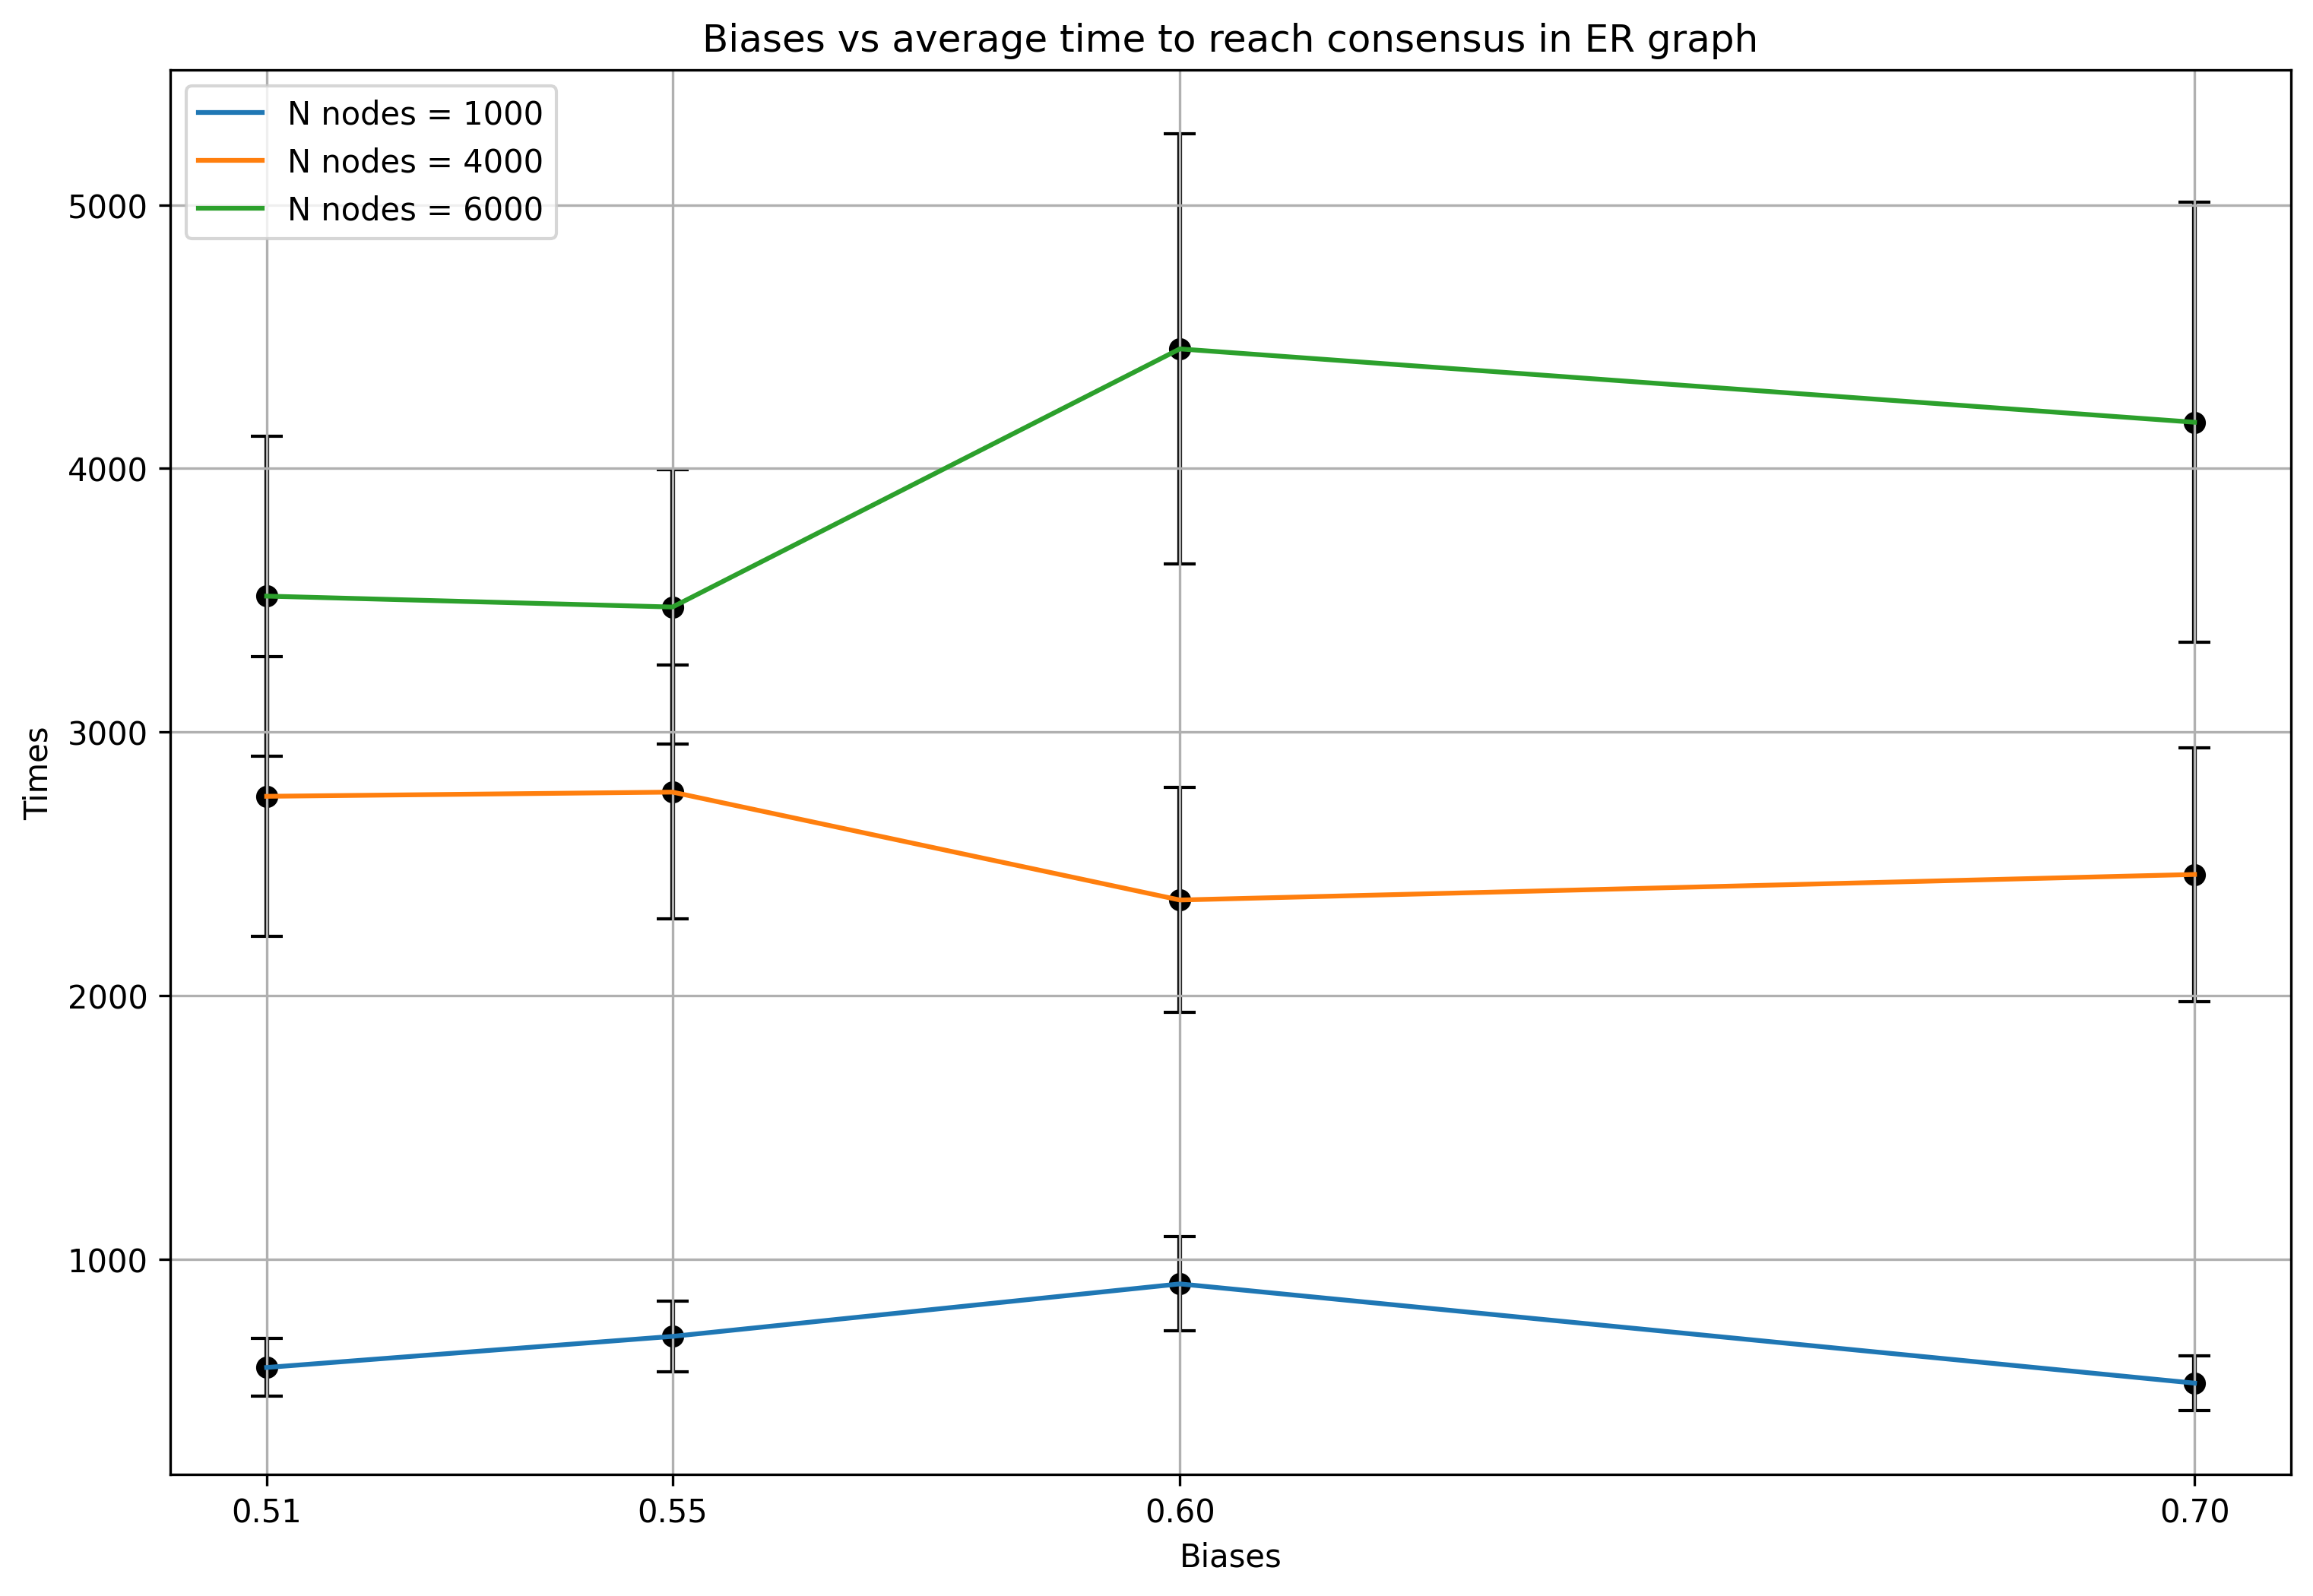
\includegraphics[width=\columnwidth]{media/er_times.png}
            \caption[short]{Average time to reach consensus based on different bias probability}
            \label{fig:er_times}
        \end{figure}

        Fig. \ref{fig:er_times} shows the analysis of the average time to converge to the final state (consensus).
        %
        It is clear that the more nodes there are in the graph, the longer it takes on average to reach consensus.
        
        The interesting result is that, contrary to what intuition would suggest, the bias probability doesn't seem to have an important effect on how quickly the system reaches consensus.
        %
        In fact, it can be observed that the confidence intervals for each set of nodes overlap with one another.

        % Looking at this graph, it can be observed that the confidence intervals (represented by the vertical lines at each data point) for each series of nodes overlap with one another. This suggests that there is not a significant difference in the average time to reach consensus at different bias levels, as the results are within each other’s range of uncertainty. In other words, the average time to reach consensus for different numbers of nodes (1000, 4000, and 6000) at various bias levels appears to be statistically similar within the given confidence intervals. This overlapping of confidence intervals indicates that the differences observed between the groups may be due to random variation rather than a true difference in the populations.

        Fig. \ref{fig:er_consensus} shows the results for the probability of the final state being a +1 consensus. 
        %
        It shows that the initial state has an influence on the type of final state the system reaches. 
        %
        In fact, there is a general trend that suggests that the higher the bias probability, the more likely the +1 consensus.
        
        It can also be seen that the differences observed between the groups are not clear enough to be attributed to reasons other than random variation. 
        %
        The lines representing each group intersect and overlap at several points on the graph, indicating that there is no clear separation or significant difference in their +1 probability as the bias probability changes. 
        %
        This suggests that the size of the graph does not have a clear effect on the +1 probability.

        \begin{figure}[!ht]
            \centering
            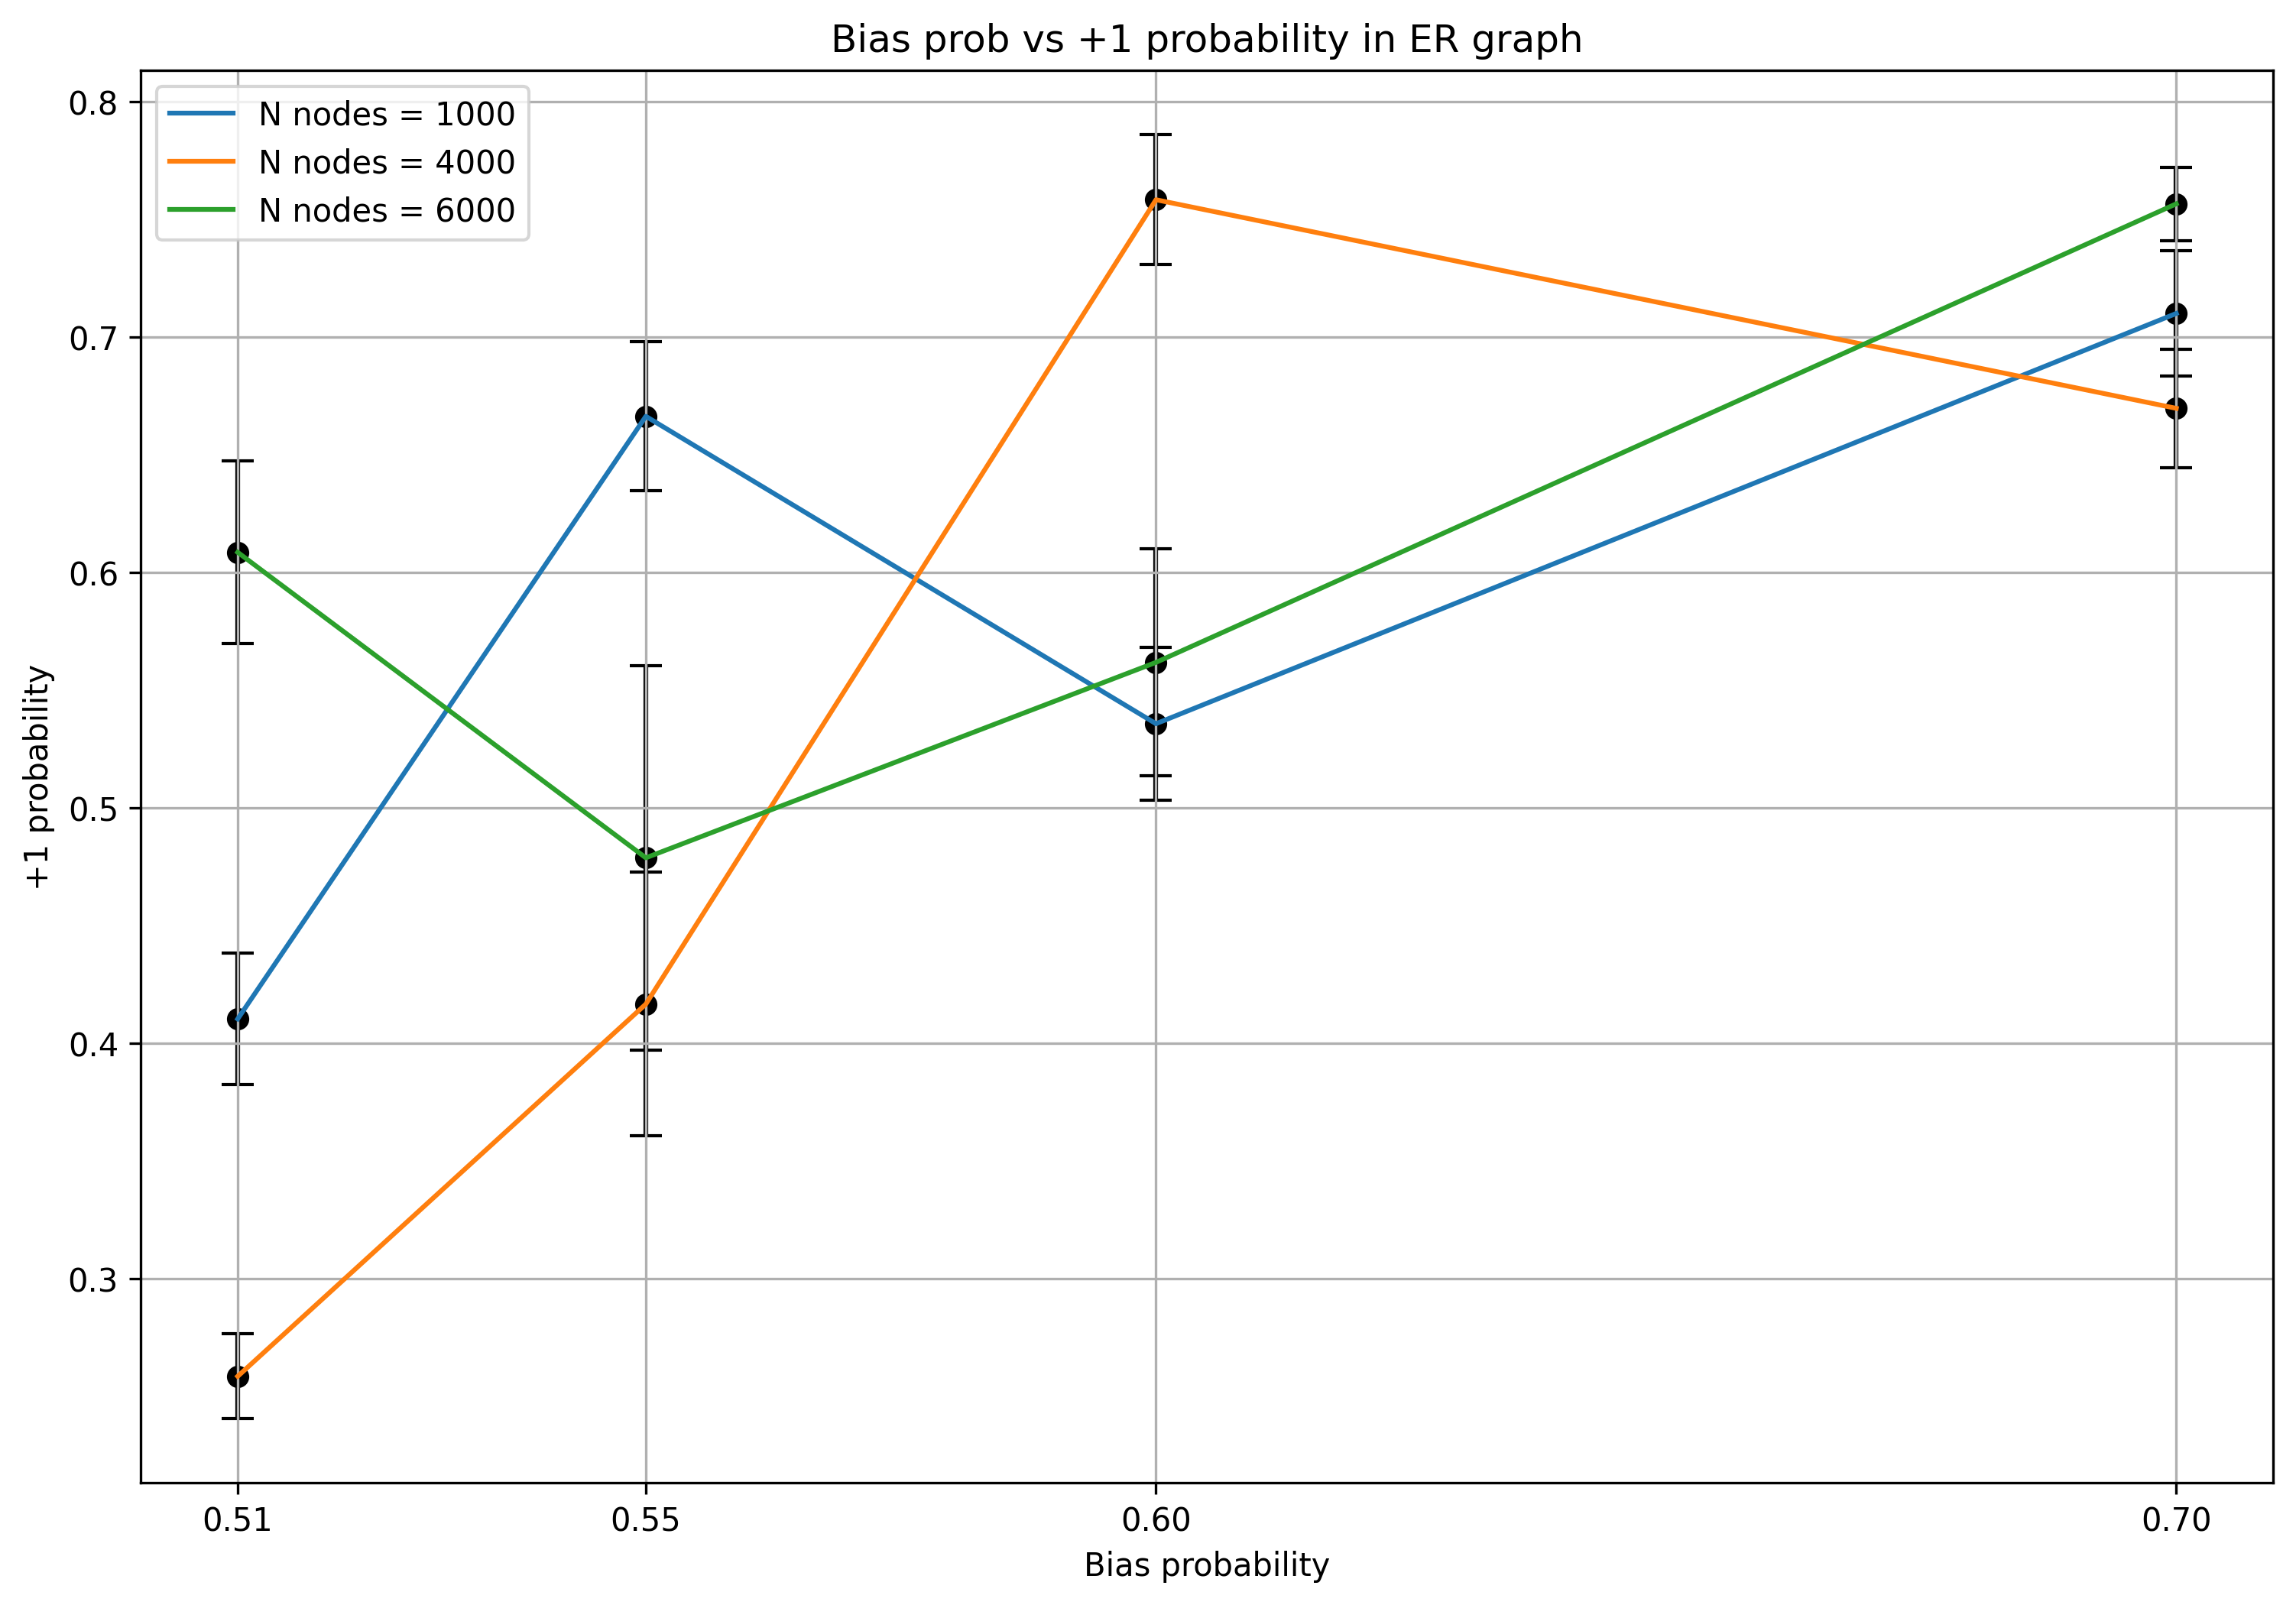
\includegraphics[width=\columnwidth]{media/er_consensus.png}
            \caption[short]{+1 probability based on different bias probability}
            \label{fig:er_consensus}
        \end{figure}

        %Looking at this graph, it can be observed that the differences between the various groups (N nodes = 1000, N nodes = 4000, N nodes = 6000) are not distinct enough to be attributed to reasons other than normal random variation. The lines representing each group intersect and overlap at several points on the graph, indicating that there is no clear separation or significant difference in their +1 probability as bias probability changes. This suggests that the variations observed in the +1 probability across different bias probabilities for each group could be due to inherent randomness in the system rather than any systematic differences between the groups. In other words, the graph does not provide strong evidence to suggest that the number of nodes in the graph has a significant impact on the +1 probability at different bias probabilities. It’s important to note, however, that this interpretation is based on the visual inspection of the graph and a more rigorous statistical analysis may be required to confirm these observations

    \subsection{$Z^k$ graphs}

        \begin{figure}[!ht]
            \centering
            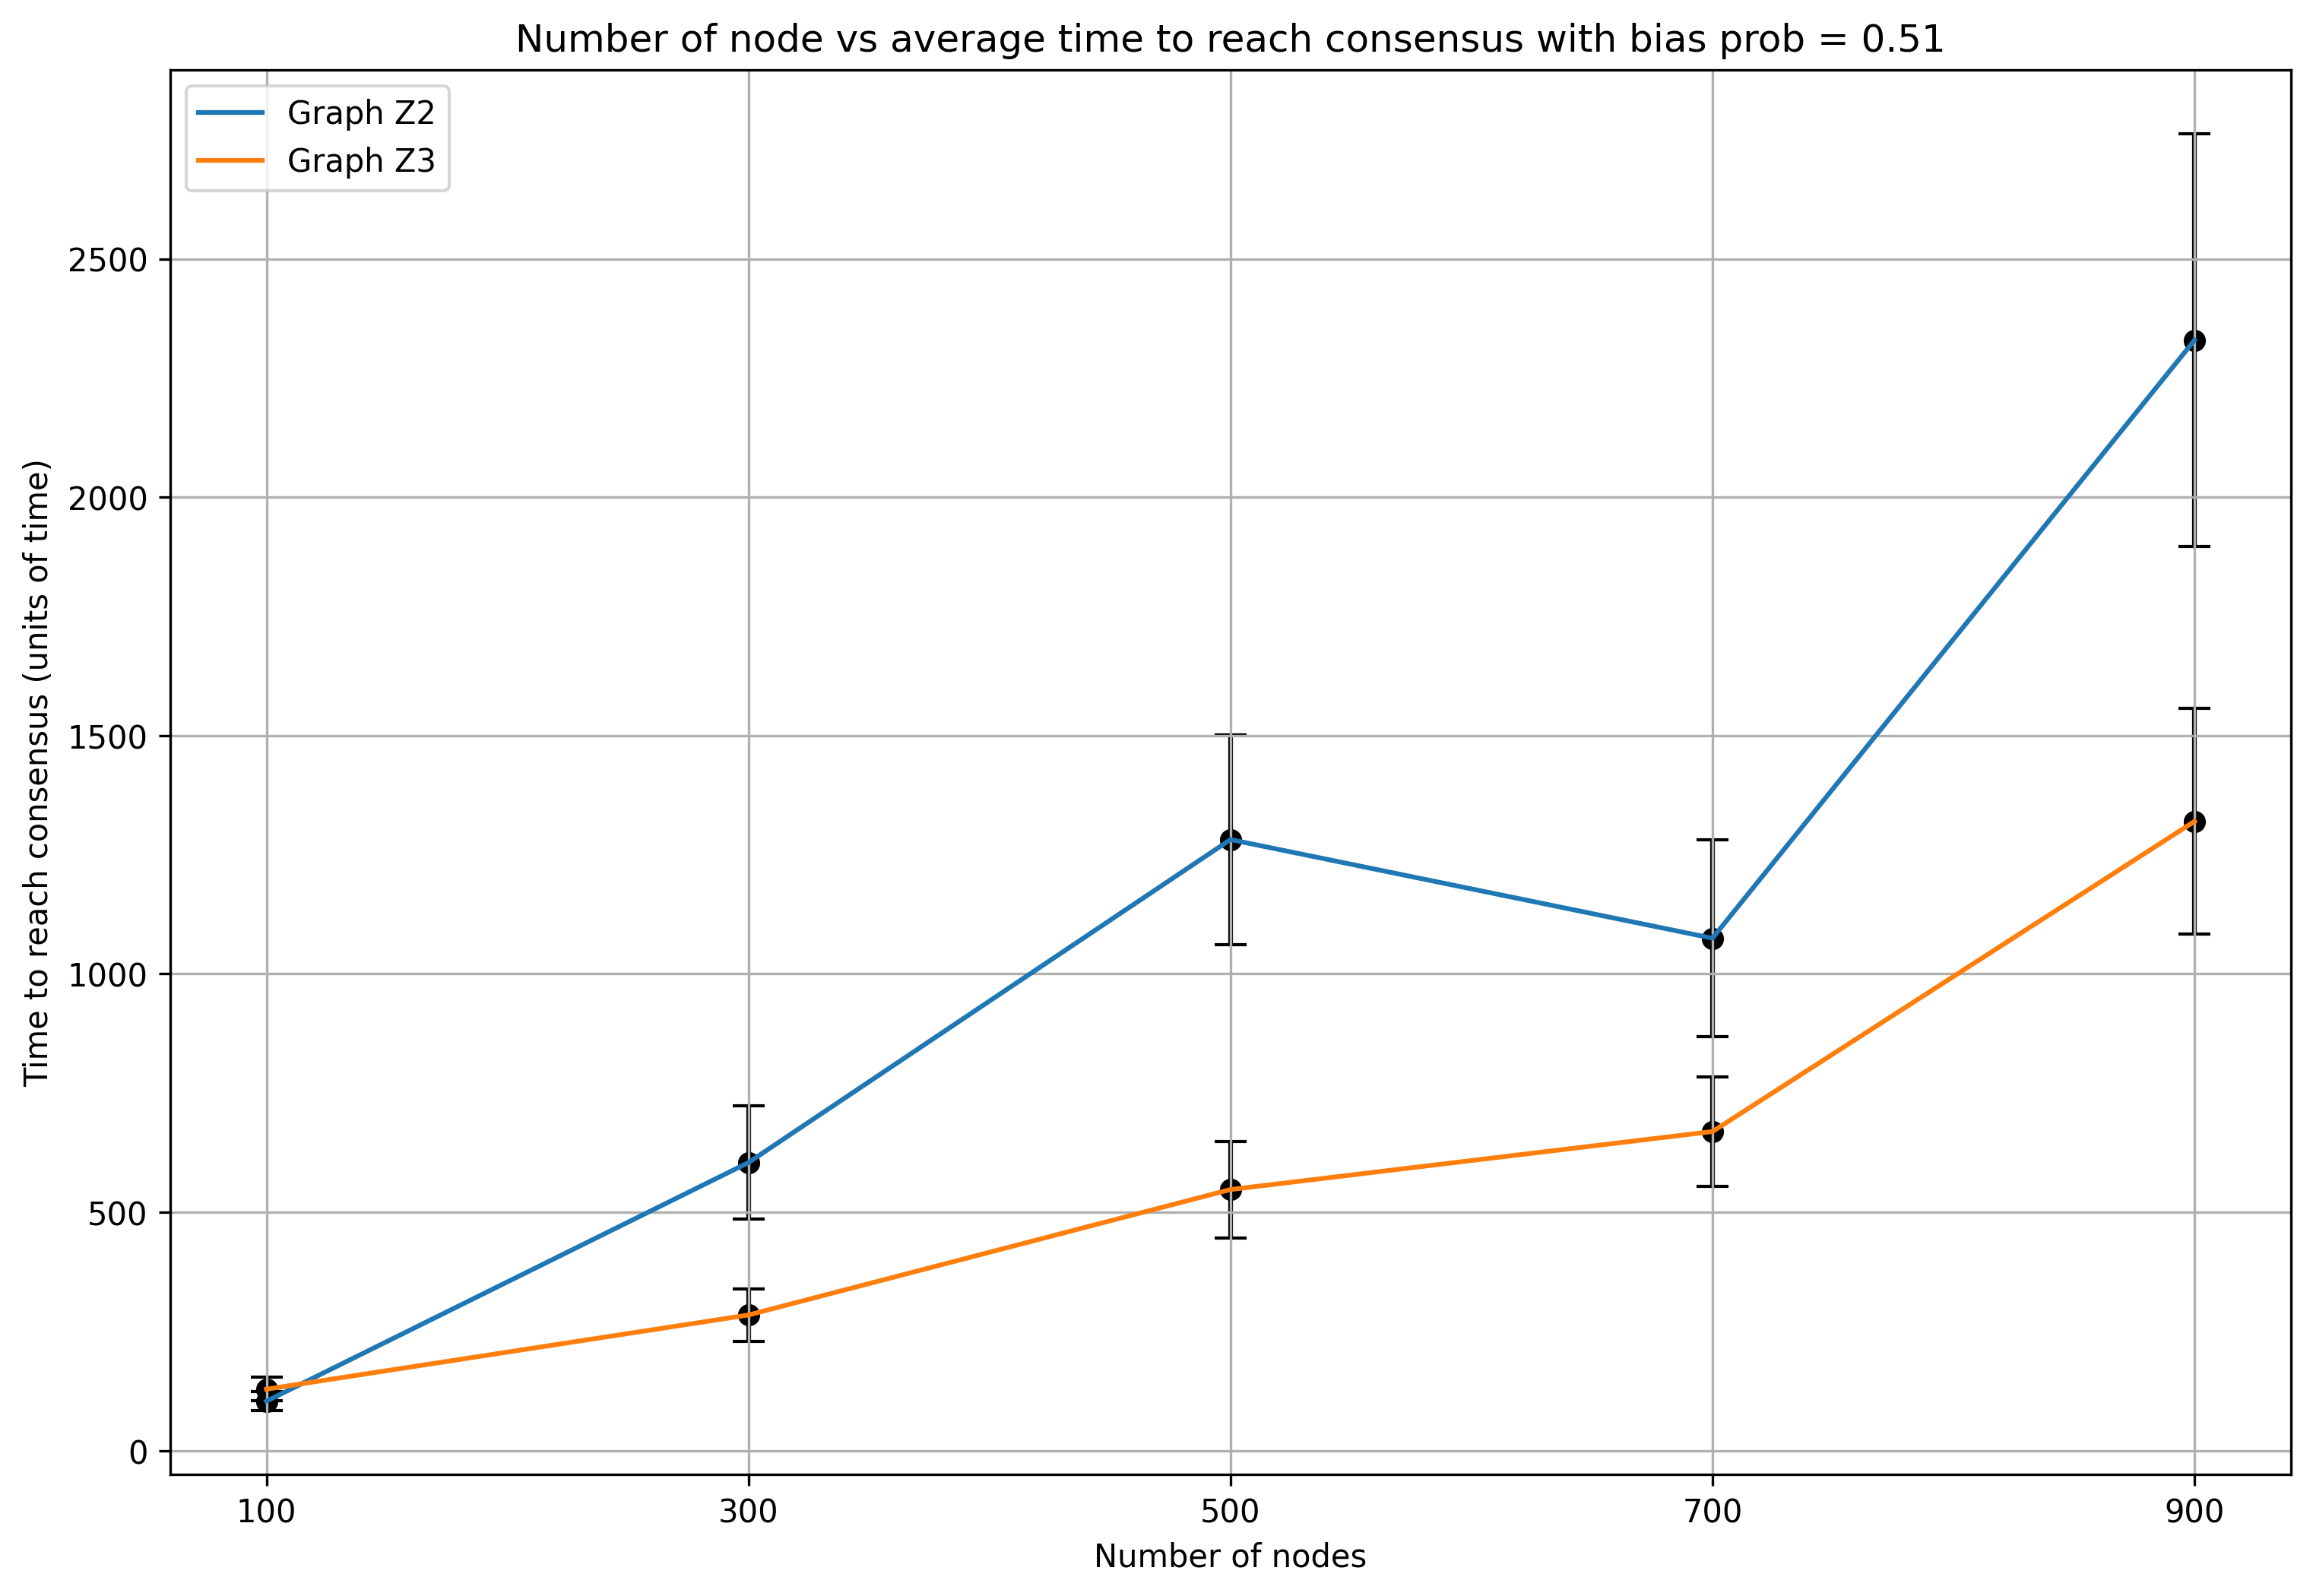
\includegraphics[width=\columnwidth]{media/z_times_bias_0.51.png}
            \caption[short]{Average time to reach consensus based on different portion of $Z^k$ graph}
            \label{fig:z_times}
        \end{figure}

        Fig. \ref{fig:z_times} clearly shows a correlation between the number of nodes in $Z^k$ graphs and the average time to reach consensus.
        %
        It can also be observed that the $Z^3$ converges faster than the $Z^2$, which can be explained by the fact that the nodes have more connections in the first case. 

        \begin{figure}[!ht]
            \centering
            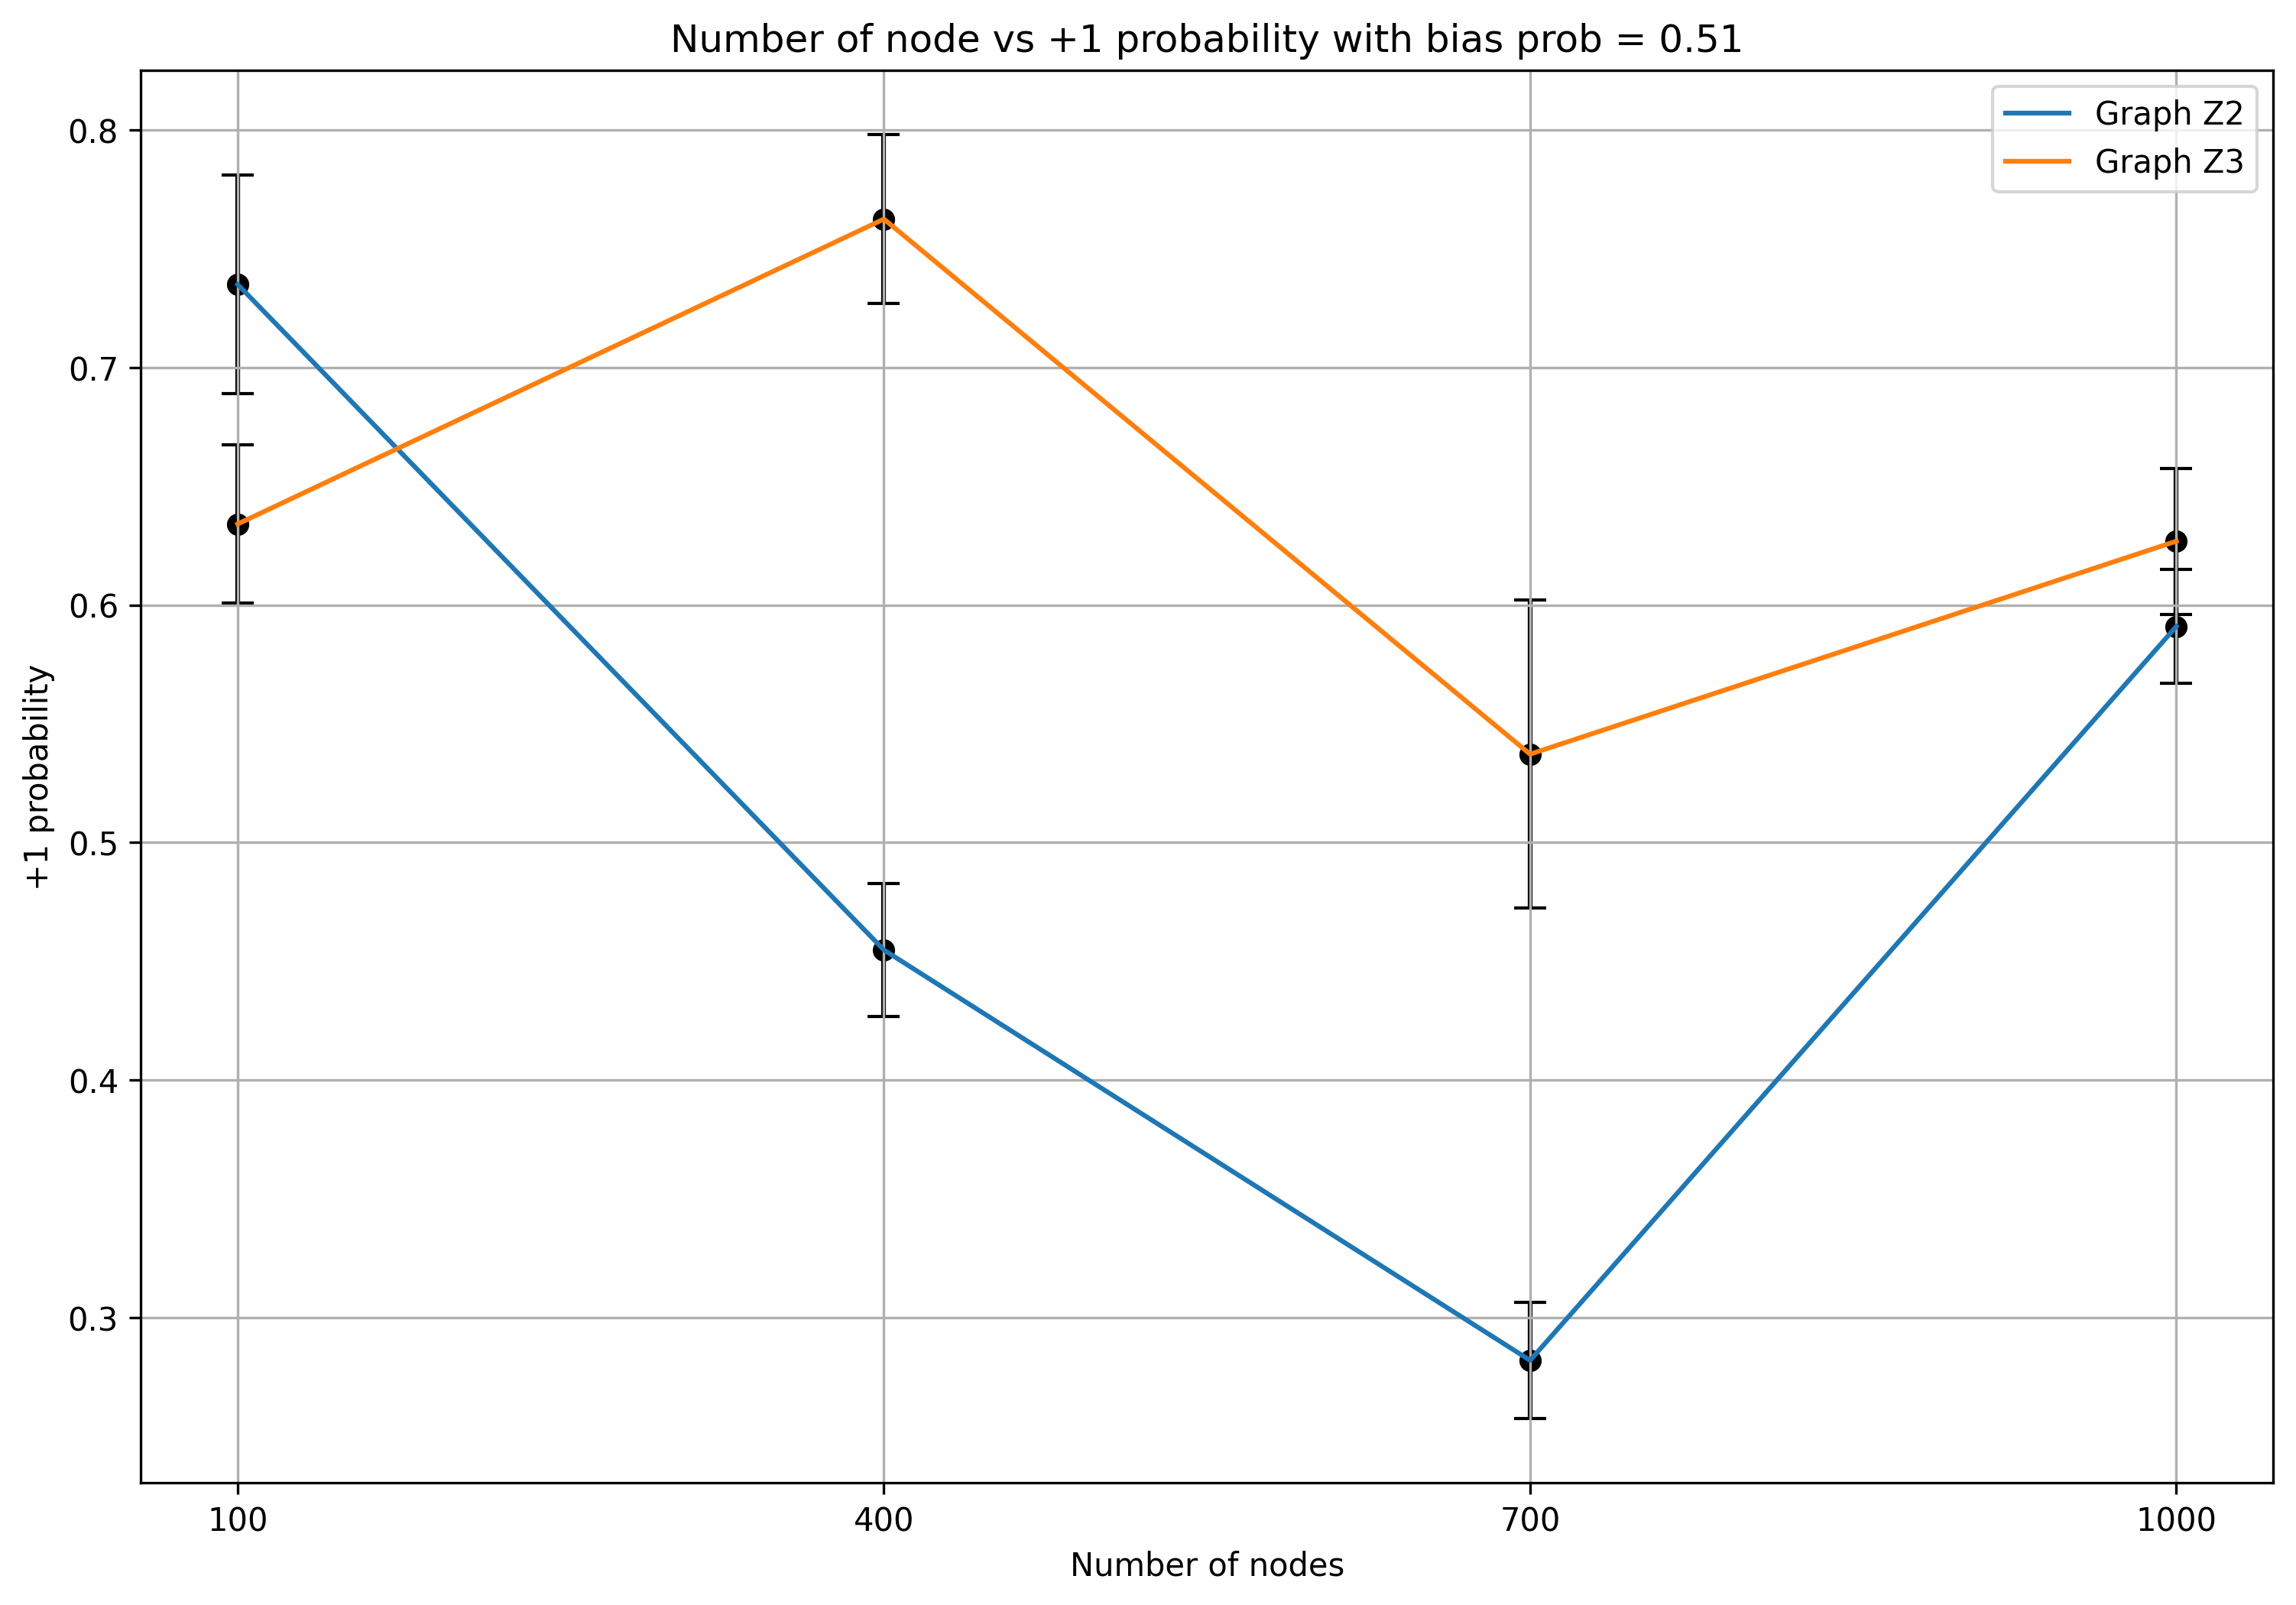
\includegraphics[width=\columnwidth]{media/z_consensus_bias_0.51.png}
            \caption[short]{+1 probability based on different portion of $Z^k$ graph}
            \label{fig:z_consensus}
        \end{figure}

        Fig. \ref{fig:z_consensus} shows that neither the size or the type of graph seems to have a direct effect on the +1 probability. In fact, there is no particular trend in the simulation that clearly separates the two groups. 

    %In Fig. \ref{fig:state_2} and \ref{fig:state_2(biased)} we can see that in the second case, it is more likely that the graph will reach a stable state starting from a biased condition. 
    
\section{Conclusion}

    In conclusion, the paper provides valuable insights into the dynamic processes on graphs. The importance of the initial bias probability on the average time to consensus has been studied, and the relative unimportance of it for the +1 probability has been shown to be consistent with theoretical predictions. 

%\bibliography{bibliography}
%\bibliographystyle{ieeetr}

\end{document}
